\documentclass[10pt,letterpaper]{article}
\usepackage[margin=0.75in]{geometry}
\usepackage[T1]{fontenc}
\usepackage{lmodern,microtype}
\usepackage{amsmath,amssymb,booktabs,graphicx}
\usepackage{float}
\usepackage[font=small,labelfont=bf]{caption}
\usepackage[hidelinks]{hyperref}
\usepackage{enumitem}
\setlist[itemize]{nosep,leftmargin=*}
\setlength{\parindent}{0pt}
\setlength{\parskip}{5pt}
\setlength{\emergencystretch}{2em}
\begin{document}
\begin{center}
{\Large\bfseries Heat effects across socioeconomic clusters}\\[3pt]
{\large Cluster-level attributable risk and posterior exceedance}\\[3pt]
September 10, 2026
\end{center}

\section*{1. Heat metric and hierarchical model}
The supplied data contain \textbf{56,856 ZIP-days}: 309 ZIPs in 14 Los Angeles socioeconomic clusters, observed May 1--October 31, 2018. The response is \texttt{D2}; population is the exposure. Supplied counts and cluster assignments are treated as fixed.

Let $T^{\max}_{it}$ denote \textbf{daily maximum heat index} (\texttt{Max\_HI\_Value}), not daily mean temperature. We standardize it as $h_{it}=(T^{\max}_{it}-\overline{T^{\max}})/s_{T^{\max}}$, using the mean and SD across all observed ZIP-days, and decompose it as $h_{it}=m_i+x_{it}$, where $m_i=\operatorname{mean}_t(h_{it})$ is ZIP $i$'s study-period mean (chronic heat) and $x_{it}$ is the daily deviation from that mean (acute heat). This daily-maximum metric is also specified in the \href{https://calheatscore.calepa.ca.gov/sites/default/files/2026-02/methods_v2.pdf}{CalHeatScore methods}, pp.~5--8; the averaging window here is May--October 2018.

\textbf{Observation and linear-predictor levels.}
\begin{equation}
\begin{aligned}
Y_{it}\mid\theta &\sim \operatorname{Poisson}(\mu_{it}),\\
\mu_{it} &= N_i\exp(\eta_{it}),\\
\eta_{it} &= \alpha_{c(i)}+\gamma m_i+\beta_{c(i)}x_{it}\\
&\quad +\mathbf z_{\mathrm{month}(t)}^\top\mathbf b_{\mathrm{month}}
       +\mathbf z_{\mathrm{weekday}(t)}^\top\mathbf b_{\mathrm{weekday}}
       +u_{\mathrm{doy}(t)},\\
\alpha_c &= \alpha+a_c,\qquad
\beta_c=\beta_0+\delta_c,\qquad a_6=\delta_6=0.
\end{aligned}
\label{eq:model}
\end{equation}
The $\mathbf z$ vectors are categorical indicators: month and weekday are \textbf{fixed effects}, with May and Sunday as references. Cluster intercept contrasts $a_c$ and slope contrasts $\delta_c$ are also fixed effects, not draws from an estimated between-cluster distribution.

\textbf{Temporal random-effect level.}
\[
p(\mathbf u\mid\tau)\ \propto\
\tau^{r/2}\exp\!\left[-\frac{\tau}{2}\mathbf u^\top Q_{\mathrm{RW2,scaled}}\mathbf u\right].
\]
Here $Q_{\mathrm{RW2,scaled}}$ is the scaled second-order random-walk structure matrix of rank $r$, with INLA's constraints imposed. The fit uses INLA defaults: $\tau\sim\operatorname{Gamma}(1,5\times10^{-5})$ (shape, rate), independent $N(0,1000)$ priors for non-intercept fixed coefficients, and a flat intercept prior. INLA provides posterior inference. A negative-binomial likelihood with the same predictor is fitted for comparison; the \textbf{Poisson posterior supplies the map}.

\section*{2. Cluster-average attributable risk}
For the $n_c$ ZIP-days in cluster $c$, define $H_c=n_c^{-1}\sum_{(i,t)\in\mathcal I_c}m_i$ and $d_{it}=h_{it}-H_c$. The counterfactual replaces standardized daily maximum heat $h_{it}$ with $H_c$, retaining $m_i$, cluster, and temporal covariates: $\eta_{it}^{\mathrm{CF}}=\eta_{it}-\beta_c d_{it}$.
The cluster estimand is the \textbf{signed average excess rate per 10,000 population per day}:
\begin{equation}
AR_c(\theta)=\frac{10^4}{n_c}
\sum_{(i,t)\in\mathcal I_c}
\left[e^{\eta_{it}}-e^{\eta_{it}-\beta_c d_{it}}\right],
\label{eq:ar}
\end{equation}
Both positive and negative ZIP-day contrasts enter this equal-weight average. It is a model-based rate contrast over the study period, not a population-weighted count of attributable visits or a contrast at one temperature.

\newpage
\section*{3. Posterior exceedance probability}
Using $S=4{,}000$ joint draws from the INLA-approximated posterior, evaluate Eq.~\eqref{eq:ar} within each draw. The mapped probability is estimated by
\begin{equation}
\pi_c=\Pr\{AR_c(\theta)>0\mid D\}
\;\approx\;\widehat\pi_c=\frac{1}{S}\sum_{s=1}^{S}
\mathbf{1}\{AR_c(\theta^{(s)})>0\}.
\label{eq:mc}
\end{equation}
Each joint draw retains dependence between linear predictors and cluster slopes. The draws also provide posterior means and 95\% equal-tailed credible intervals for $AR_c$. Sampling uses seed 20260910 and batches of 200; estimates of zero or one mean none or all of the 4,000 draws exceed zero, not posterior certainty.

\section*{4. Socioeconomic cluster profiles}
Figure~\ref{fig:cluster-profiles} summarizes the 20 supplied covariates for the same 309 ZCTAs used in the analysis; no clusters are re-estimated. For variable $j$, let $q_{cj}$ be its median across ZCTAs in cluster $c$. The heatmap shows $z_{cj}=(q_{cj}-\bar q_{\cdot j})/s_j$, where $\bar q_{\cdot j}$ and $s_j$ are the unweighted mean and sample SD of the 14 cluster medians (SD denominator 13). Neither the medians nor their standardization use population weights.

\begin{figure}[H]
\centering
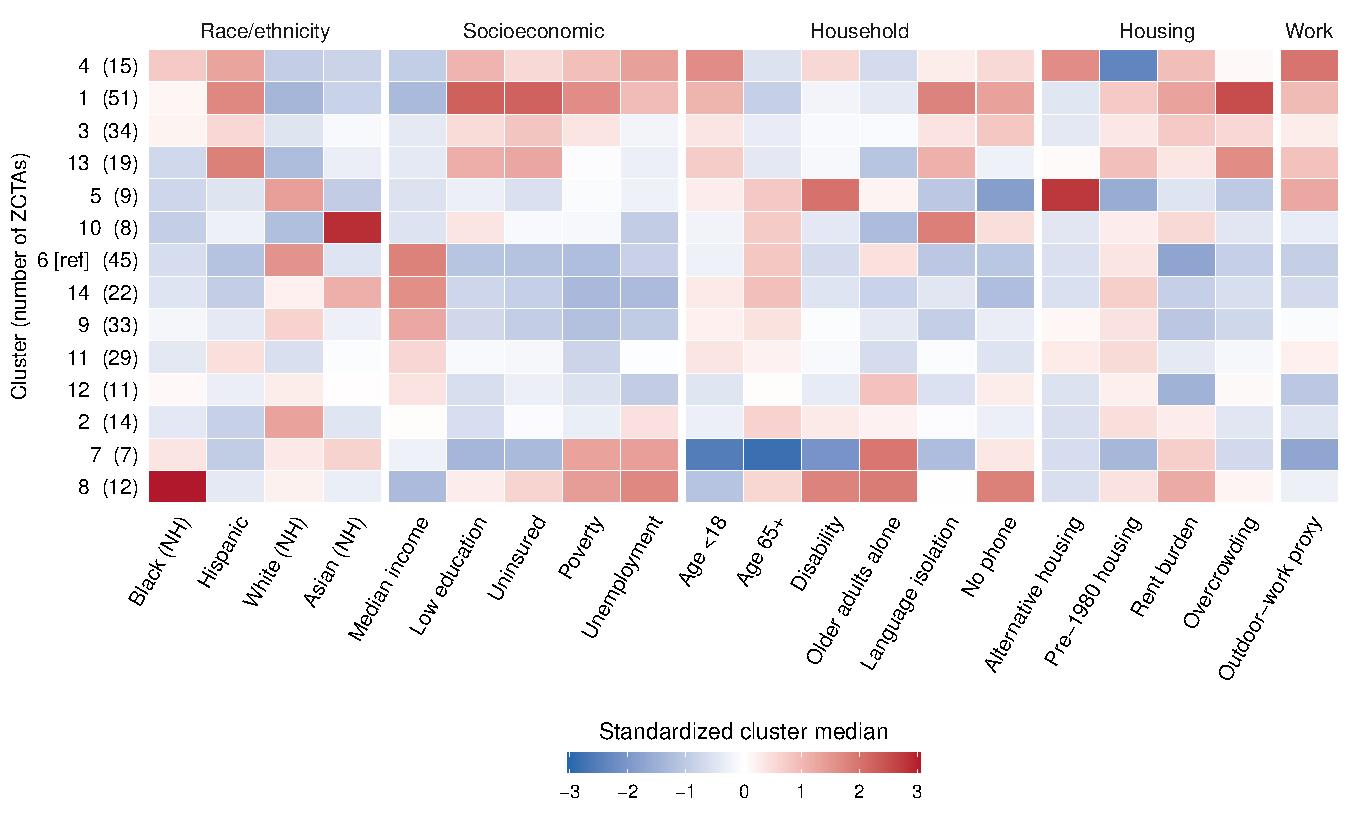
\includegraphics[width=\linewidth]{ses_clusters-main/Los_Angeles_discrete_none_HEAT_by_cluster/cluster_profiles_heatmap.pdf}
\caption{Socioeconomic and demographic profiles of the 14 Los Angeles clusters. Cells show standardized within-cluster medians, $z_{cj}$, with blue, white, and red indicating values below, at, and above the across-cluster mean of medians. Red means a higher covariate value, not necessarily greater vulnerability; income and other variables retain their original direction. Gray denotes missing or undefined standardized values. Rows are ordered by profile similarity, and columns by similarity within each theme. Parentheses give ZCTA counts and [ref] marks reference cluster 6; NH denotes non-Hispanic.}
\label{fig:cluster-profiles}
\end{figure}

Rows and within-theme columns follow Ward's hierarchical dendrogram leaf order (\texttt{ward.D2}, Euclidean distance). Row distances use the 20 standardized covariates; column distances use the 14 cluster profiles. This is a similarity arrangement, not a risk ranking; cluster assignments, reference, and values are unchanged. \texttt{cluster\_profiles\_heatmap.csv} records the values, scaling parameters, and display orders.

\newpage
\section*{5. Results and model assessment}
\begin{center}
\begin{tabular}{lrr}
\toprule
Diagnostic & Poisson & Negative binomial\\
\midrule
WAIC (lower is better) & 93,408.42 & 65,425.64\\
Plug-in predicted zero fraction & 75.88\% & 87.52\%\\
Observed zero fraction & 87.65\% & 87.65\%\\
\bottomrule
\end{tabular}
\end{center}
The negative-binomial size estimate is approximately $0.10$. Its lower WAIC and closer zero fraction support further consideration of that likelihood; full posterior-predictive assessment remains necessary.

Exceedance probabilities exceed 99\% in clusters 1, 3, 4, 11, and 13; they are 0.825\% in cluster 6, 0/4,000 positive draws in cluster 8, and 12.425\% in cluster 14. Cluster 8 has mean $AR_c=-0.05387$ per 10,000 per day (95\% credible interval: $-0.11280$ to $-0.01703$). Positive slopes need not imply positive aggregate contrasts.

Figure~\ref{fig:ar-exceedance} maps the cluster-level exceedance probabilities; each mapped ZCTA inherits its cluster's estimate.
\begin{figure}[H]
\centering

\includegraphics[height=3.5in]{ses_clusters-main/Los_Angeles_discrete_none_HEAT_by_cluster/AR_gt_0_gradient.png}
\caption{Posterior probability of a positive cluster-average excess rate in mainland Los Angeles, May--October 2018. Colors show estimates of $\pi_c=\Pr\{AR_c(\theta)>0\mid D\}$, where $D$ denotes the observed data and $AR_c(\theta)$ is the signed mean rate contrast against the cluster-mean heat reference (Eq.~\eqref{eq:ar}). Probabilities are estimated from 4,000 joint draws of the INLA-approximated Poisson posterior (model in Eq.~\eqref{eq:model}), using the exceedance estimator in Eq.~\eqref{eq:mc}. Blue, white, and red indicate 0\%, 50\%, and 100\%, respectively. Gray denotes missing estimates or areas without ZCTA coverage. Islands are omitted from the display only; estimates use the full study data.}
\label{fig:ar-exceedance}
\end{figure}

\textbf{Interpretation.} These model-based contrasts condition on the supplied clusters and imputed counts; clustering and suppression uncertainty are not propagated. Causal attribution requires additional assumptions. Individual coefficient probabilities use \texttt{inla.pmarginal}. Statewide risk cutoffs and temperature thresholds remain separate analyses.

{\footnotesize\textbf{Reproducibility.} R 4.2.3; INLA 23.4.11.1. Analysis and sampling: \path{ses_clusters-main/hri_ed.R} and \path{ses_clusters-main/cluster_ar.R}. Run \texttt{create\_map.R} in the cluster output directory to regenerate both figures and the heatmap CSV from saved analysis outputs. That directory also contains posterior draws/settings; \texttt{snapshot.json} records provenance.}
\end{document}
